\documentclass[letterpaper, 10 pt, journal, twoside]{ieeetran}
\IEEEoverridecommandlockouts

\usepackage{pdflscape}
\graphicspath{{./images/}}
\usepackage{amsfonts}
\usepackage{booktabs}
\usepackage{multirow}
\usepackage{amsmath}
\usepackage{bm}
\usepackage{hyperref}
\hypersetup{
    colorlinks=true,
    linkcolor=blue,
    filecolor=magenta,      
    urlcolor=cyan,
    pdftitle={Overleaf Example},
    pdfpagemode=FullScreen,
    }
\usepackage[export]{adjustbox}
\usepackage[normalem]{ulem}
\usepackage{tabularx,ragged2e,caption}
\usepackage{array}
\usepackage[style=ieee,sorting=none,backend=bibtex]{biblatex}
\addbibresource{./ref.bib}
\newcolumntype{A}{>{\arraybackslash}m{3em}}
\newcolumntype{B}{>{\centering\arraybackslash}m{1em}}
\newcolumntype{C}{>{\centering\arraybackslash}m{2em}}
\newcolumntype{D}{>{\centering\arraybackslash}m{5.5em}}
\newcolumntype{E}{>{\arraybackslash}m{21em}}
\newcolumntype{F}{>{\arraybackslash}m{0.95\columnwidth}}
\newcommand{\rp}[1]{\textcolor{black}{#1}}
\newcommand{\rps}[1]{\textcolor{red}{#1}}
\newcommand{\zj}[1]{\textcolor{blue}{#1}}

\renewcommand{\thesection}{S.\Roman{section}}
\renewcommand{\theequation}{S.\arabic{equation}}
\renewcommand{\thefigure}{S.\arabic{figure}}

\usepackage{caption}
\usepackage{subcaption}
\maxdeadcycles=200

\title{\LARGE \bf
DDBot: Differentiable Physics-based Digging Robot for Unknown Granular - Supplementary Materials
}

\author{Xintong Yang$^{1}$, Minglun Wei$^{1}$, Yu-Kun Lai$^{2}$, Ze Ji$^{1}$% <-this % stops a space
\thanks{}% <-this % stops a space
\thanks{$^{1}$Xintong Yang, Minglun Wei and Ze Ji are with the School of Engineering, Cardiff University, Cardiff, United Kingdom. {\tt\small \{yangx66, weim9, jiz1\}@cardiff.ac.uk}}%
\thanks{$^{2}$Yu-Kun Lai is with the School of Computer Science and Informatics, Cardiff University, Cardiff, United Kingdom. {\tt\small laiy4@cardiff.ac.uk}}%
}

\begin{document}


\maketitle
\thispagestyle{empty}
\pagestyle{empty}

%%%%%%%%%%%%%%%%%%%%%%%%%%%%%%%%%%%%%%%%%%%%%%%%%%%%%%%%%%%%%%%%%%%%%%%%%%%%%%%%

\section{Gradients of the skill parameters from actions through the skill-to-action mapping}
\rp{This subsection presents the gradient chain of the skill-to-action mapping function, which is defined mathematically by Eqs. 8 to 22. We are concerned of the gradients $\frac{\partial \bar{a}(\pmb{\theta})}{\partial \pmb{\theta}}$. The following derives the gradient of each parameter from phases 1 to 4, assuming the calculation of a rounded number of timesteps is adopted. For phases 1 and 4, the alternative approach of using a unrounded number of timesteps in per-action displacement calculation is also presented. Please also refer to Table I for math notations.}

\rp{The first parameter, $\theta_{dispalce}$, is involved in computing only the first phase of the skill actions. Thus, with $T_1=0$ ($\theta_{dispalce}=\theta_{rotate}=0$), $\frac{\partial \bar{a}}{\partial \theta_{dispalce}}=\frac{\partial \bar{a}[0:T_1]}{\partial \theta_{dispalce}}=0$. Then, because $a_t$ is the same within each phase, for any timestep $t$ that satisfies $T_1>t>0$, we have:}

\begingroup\makeatletter\def\f@size{8}\check@mathfonts\rp{\vspace{-0.3cm}
\begin{flalign*}
&\frac{\partial \bar{a}[0:T_1]}{\partial \theta_{displace}}\Bigg|_{rounded\_T_1}=\sum_{t=0}^{T_1}\frac{\partial a_t}{\partial \theta_{displace}}=T_1\cdot\frac{\partial a_t}{\partial \Delta x_1}\cdot\frac{\partial\Delta x_1}{\partial d_1}\cdot\frac{\partial d_1}{\partial \theta_{displace}}&&
\end{flalign*}}
\endgroup\vspace{-0.3cm}

\noindent \rp{where,}

\begingroup\makeatletter\def\f@size{8}\check@mathfonts\rp{\vspace{-0.3cm}
\begin{flalign*}
&\frac{\partial a_t}{\partial \Delta x_1}=\frac{\text{d} a_t[0]}{\text{d} \Delta x_1}=1,\ \ \frac{\partial\Delta x_1}{\partial d_1}=\frac{\text{d}\Delta x_1}{\text{d} d_1}=\frac{1}{T_1}, && \\
&\frac{\partial d_1}{\partial \theta_{displace}}=\frac{\text{d}d_1}{\text{d}\theta_{displace}}=0.12&&
\end{flalign*}}
\endgroup\vspace{-0.3cm}

\rp{Thus, the gradient of $\theta_{dispalce}$ with the rounded number of timesteps being used in skill-to-action mapping is:}

\begingroup\makeatletter\def\f@size{8}\check@mathfonts\rp{\vspace{-0.3cm}
\begin{flalign*}
&\frac{\partial \bar{a}[0:T_1]}{\partial \theta_{displace}}\Bigg|_{rounded\_T_1}=0.12&&
\end{flalign*}}
\endgroup\vspace{-0.3cm}

\rp{If $T_1$ is replaced with the unrounded $T^{float}_1$ to compute the per-step action, for any timestep $t$ that satisfies $T_1>t>0$, we have:}

\begingroup\makeatletter\def\f@size{8}\check@mathfonts\rp{\vspace{-0.3cm}
\begin{flalign*}
&\hspace{-0.5cm}\frac{\partial \bar{a}[0:T_1]}{\partial \theta_{displace}}\Bigg|_{unrounded\_T_1}=\sum_{t=0}^{T_1}\frac{\partial a_t}{\partial \theta_{displace}}&&\\
=&T_1\cdot\left[\frac{\partial a_t}{\partial \Delta x_1}\cdot\frac{\partial\Delta x_1}{\partial \theta_{displace}}+\frac{\partial a_t}{\partial \Delta rx_1}\cdot\frac{\partial\Delta rx_1}{\partial \theta_{displace}}\right]&&\\
=&T_1\cdot\left[\frac{\partial a_t}{\partial \Delta x_1}\cdot(\frac{\partial\Delta x_1}{\partial d_1}\cdot\frac{\partial d_1}{\partial \theta_{displace}}+\frac{\partial\Delta x_1}{\partial T^{float}_1}\cdot\frac{\partial T^{float}_1}{\partial \theta_{displace}})\right.&&\\
&\left.+\frac{\partial a_t}{\partial \Delta rx_1}\cdot\frac{\partial\Delta rx_1}{\partial T^{float}_1}\cdot\frac{\partial T^{float}_1}{\partial \theta_{displace}}\right]&&
\end{flalign*}}
\endgroup\vspace{-0.3cm}

\noindent \rp{where,}

\begingroup\makeatletter\def\f@size{8}\check@mathfonts\rp{\vspace{-0.3cm}
\begin{flalign*}
&\frac{\partial\Delta x_1}{\partial d_1}=\frac{\text{d}\Delta x_1}{\text{d} d_1}=\frac{1}{T^{float}_1},&&\\
&\frac{\partial\Delta x_1}{\partial T^{float}_1}=\frac{\text{d}\Delta x_1}{\text{d} T^{float}_1}=\frac{-d_1}{(T^{float}_1)^2},&&\\
&\frac{a_t}{\Delta rx_1}=1,\ \ \frac{\partial\Delta rx_1}{\partial T^{float}_1}=\frac{\text{d}\Delta rx_1}{\text{d} T^{float}_1}=\frac{-\varphi_1}{(T^{float}_1)^2}&&\\
&\frac{\partial T^{float}_1}{\partial \theta_{displace}}=
    \begin{cases}
        \frac{\partial T^{float}_{d_1}}{\partial |d_1|}\cdot\frac{\partial |d_1|}{\partial \theta_{displace}}, &T^{float}_{d_1}\geq T^{float}_{\varphi_1}>0\\
        \frac{\partial T^{float}_{\varphi_1}}{\partial \theta_{displace}}=0, &0<T^{float}_{d_1}<T^{float}_{\varphi_1}
    \end{cases},&&\\
\end{flalign*}}
\endgroup\vspace{-0.3cm}

\noindent \rp{where,}

\begingroup\makeatletter\def\f@size{8}\check@mathfonts\rp{\vspace{-0.3cm}
\begin{flalign*}
&\frac{\partial T^{float}_{d_1}}{\partial |d_1|}=\frac{1}{v_l\cdot\Delta t},\ \ \frac{\partial |d_1|}{\partial \theta_{displace}}=\begin{cases}
    0.12, &\theta_{displace}>0\\
    -0.12, &\theta_{displace}<0\\
    0, &\theta_{displace}=0
    \end{cases}&&
\end{flalign*}}
\endgroup\vspace{-0.3cm}

\rp{Thus, we have}
\begingroup\makeatletter\def\f@size{8}\check@mathfonts\rp{\vspace{-0.3cm}
\begin{flalign*}
    &\frac{\partial \bar{a}[0:T_1]}{\partial \theta_{displace}}\Bigg|_{unrounded\_T_1}&&\\
    &=\begin{cases}
    T_1\cdot\left[1\cdot(\frac{1}{T^{float}_{d_1}}\cdot0.12 + \frac{-d_1}{(T^{float}_{d_1})^2}\cdot\frac{1}{v_l\cdot\Delta t}\cdot0.12)\right.\\
    \hspace{0.2cm}\left.+1\cdot\frac{-\varphi_1}{(T^{float}_{d_1})^2}\cdot\frac{1}{v_l\cdot\Delta t}\cdot0.12\right],\\
    \hspace{3cm} T^{float}_{d_1}\geq T^{float}_{\varphi_1}>0,\ \theta_{displace}>0\\
    T_1\cdot\left[1\cdot(\frac{1}{T^{float}_{d_1}}\cdot0.12 + \frac{-d_1}{(T^{float}_{d_1})^2}\cdot\frac{1}{v_l\cdot\Delta t}\cdot-0.12)\right.\\
    \hspace{0.2cm}\left.+1\cdot\frac{-\varphi_1}{(T^{float}_{d_1})^2}\cdot\frac{1}{v_l\cdot\Delta t}\cdot-0.12\right],\\ 
    \hspace{3cm} T^{float}_{d_1}\geq T^{float}_{\varphi_1}>0,\ \theta_{displace}<0\\
    T_1\cdot1\cdot\frac{1}{T^{float}_{\varphi_1}}\cdot0.12,\hspace{0.35cm}0<T^{float}_{d_1}<T^{float}_{\varphi_1}
    \end{cases}&&\\
    &=\begin{cases}
    T_1\cdot\frac{-\pi\cdot\theta_{rotate}\cdot v_l\cdot\Delta t}{0.36\cdot{\theta_{displace}}^2},\ \ T^{float}_{d_1}\geq T^{float}_{\varphi_1}>0,\ \theta_{displace}>0\\
    T_1\cdot\left(\frac{2\cdot v_l\cdot\Delta t}{\theta_{displace}}+\frac{\pi\cdot\theta_{rotate}\cdot v_l\cdot\Delta t}{0.36\cdot{\theta_{displace}}^2}\right),\\
    \hspace{3cm} T^{float}_{d_1}\geq T^{float}_{\varphi_1}>0,\ \theta_{displace}<0\\
    T_1\cdot\frac{0.12\cdot v_w\cdot\Delta t}{|\theta_{rotate}|\cdot\pi/3},\hspace{0.7cm} 0<T^{float}_{d_1}<T^{float}_{\varphi_1}
    \end{cases}&&
\end{flalign*}}
\endgroup\vspace{-0.3cm}

\rp{Secondly, as $\theta_{rotate}$ is involved in the computation of skill phases 1, 2 and 4, its gradient is $\frac{\partial \bar{a}}{\partial \theta_{rotate}}=\frac{\partial \bar{a}[0:T_1]}{\partial \theta_{rotate}}+\frac{\partial \bar{a}[T_1:T_1+T_2]}{\partial \theta_{rotate}}+\frac{\partial \bar{a}[T_1+T_2+T_3:T_1+T_2+T_3+T_4]}{\partial \theta_{rotate}}$. Again, with $T_1=0$ ($\theta_{dispalce}=\theta_{rotate}=0$), we have $\frac{\partial \bar{a}[0:T_1]}{\partial \theta_{rotate}}=0$. Then, for any timestep $t$ that satisfies $T_1>t>0$, we have:}

\begingroup\makeatletter\def\f@size{8}\check@mathfonts\rp{\vspace{-0.3cm}
\begin{flalign*}
    \frac{\partial \bar{a}[0:T_1]}{\partial \theta_{rotate}}\Bigg|_{rounded\_T_1}&=T_1\cdot\frac{\partial a_t}{\partial \Delta rx_1}\cdot\frac{\partial \Delta rx_1}{\partial \varphi_1}\cdot\frac{\partial \varphi_1}{\partial \theta_{rotate}}=\frac{\pi}{3}
\end{flalign*}}
\endgroup\vspace{-0.3cm}

\rp{Again, if $T_1$ is replaced with the unrounded value, we have}

\begingroup\makeatletter\def\f@size{8}\check@mathfonts\rp{\vspace{-0.3cm}
\begin{flalign*}
    &\frac{\partial \bar{a}[0:T_1]}{\partial \theta_{rotate}}\Bigg|_{unrounded\_T_1}&&\\
    &=T_1\cdot\left[\frac{\partial a_t}{\partial \Delta rx_1}\cdot(\frac{\partial \Delta rx_1}{\partial \varphi_1}\cdot\frac{\partial \varphi_1}{\partial \theta_{rotate}}+\frac{\partial \Delta rx_1}{\partial T^{float}_1}\cdot\frac{\partial T^{float}_1}{\partial \theta_{rotate}})\right.&&\\
    &\left.+\frac{\partial a_t}{\partial \Delta x_1}\cdot\frac{\partial\Delta x_1}{\partial T^{float}_1}\cdot\frac{\partial T^{float}_1}{\partial \theta_{rotate}}\right]&&
\end{flalign*}}
\endgroup\vspace{-0.3cm}

\noindent\rp{where,}

\begingroup\makeatletter\def\f@size{8}\check@mathfonts\rp{\vspace{-0.3cm}
\begin{flalign*}
&\frac{\partial\Delta rx_1}{\partial \varphi_1}=\frac{\text{d}\Delta rx_1}{\text{d} \varphi_1}=\frac{1}{T^{float}_1},&&\\
&\frac{\partial T^{float}_1}{\partial \theta_{rotate}}=
    \begin{cases}
        \frac{\partial T^{float}_{\varphi_1}}{\partial \theta_{rotate}}=0, &T^{float}_{d_1}\geq T^{float}_{\varphi_1}>0\\
        \frac{\partial T^{float}_{d_1}}{\partial |\varphi_1|}\cdot\frac{\partial |\varphi_1|}{\partial \theta_{rotate}}, &0<T^{float}_{d_1}<T^{float}_{\varphi_1}
    \end{cases},&&\\
&\frac{\partial T^{float}_{d_1}}{\partial |\varphi_1|}=\frac{1}{v_w\cdot\Delta t},\ \ \frac{\partial |\varphi_1|}{\partial \theta_{rotate}}=\begin{cases}
    \pi/3, &\theta_{rotate}>0\\
    -\pi/3, &\theta_{rotate}<0\\
    0, &\theta_{rotate}=0
    \end{cases}&&
\end{flalign*}}
\endgroup\vspace{-0.3cm}

\rp{Thus,}

\begingroup\makeatletter\def\f@size{8}\check@mathfonts\rp{\vspace{-0.3cm}
\begin{flalign*}
    &\frac{\partial \bar{a}[0:T_1]}{\partial \theta_{rotate}}\Bigg|_{unrounded\_T_1}&&\\
    &=\begin{cases}
    T_1\cdot\left[1\cdot(\frac{1}{T^{float}_{\varphi_1}}\cdot\frac{\pi}{3} + \frac{-\varphi_1}{(T^{float}_1)^2}\cdot\frac{1}{v_w\cdot\Delta t}\cdot\frac{\pi}{3})\right.\\
    \hspace{0.2cm} \left.+1\cdot \frac{-d_1}{(T^{float}_{\varphi_1})^2}\cdot\frac{\pi/3}{v_w\cdot\Delta t}\right],\\
    \hspace{2.9cm} T^{float}_{\varphi_1}>T^{float}_{d_1}>0,\ \theta_{rotate}>0\\
    T_1\cdot\left[1\cdot(\frac{1}{T^{float}_{\varphi_1}}\cdot\frac{\pi}{3} + \frac{-\varphi_1}{(T^{float}_1)^2}\cdot\frac{1}{v_w\cdot\Delta t}\cdot-\frac{\pi}{3}))\right.,\\ 
    \hspace{0.2cm} \left.+1\cdot \frac{-d_1}{(T^{float}_{\varphi_1})^2}\cdot\frac{-\pi/3}{v_w\cdot\Delta t}\right],\\
    \hspace{2.9cm} T^{float}_{\varphi_1}>T^{float}_{d_1}>0,\ \theta_{rotate}<0\\
    T_1\cdot1\cdot\frac{1}{T^{float}_{d_1}}\cdot\frac{\pi}{3},\hspace{0.5cm}T^{float}_{\varphi_1}\leq T^{float}_{d_1}
    \end{cases}&&\\
    &=\begin{cases}
    T_1\cdot\frac{-0.36\cdot\theta_{displace}\cdot v_w\cdot\Delta t}{{\theta_{rotate}}^2\cdot\pi},\\
    \hspace{2.9cm} T^{float}_{\varphi_1}>T^{float}_{d_1}>0,\ \theta_{rotate}>0\\
    T_1\cdot\left(\frac{2\cdot v_w\Delta t}{\theta_{rotate}}+\frac{0.36\cdot\theta_{displace}\cdot v_w\cdot\Delta t}{{\theta_{rotate}}^2\cdot\pi}\right),\\
    \hspace{2.9cm} T^{float}_{\varphi_1}>T^{float}_{d_1}>0,\ \theta_{rotate}<0\\
    T_1\cdot\frac{\frac{\pi}{3}\cdot v_l\cdot\Delta t}{|\theta_{displace}|\cdot0.12},\hspace{0.4cm} 0<T^{float}_{\varphi_1}\leq T^{float}_{d_1}
    \end{cases}&&
\end{flalign*}}
\endgroup\vspace{-0.3cm}

\rp{Note that we assume $T^{float}_{1}=T^{float}_{d_1}$ when $T^{float}_{d_1}=T^{float}_{\varphi_1}$ for the $max()$ operation (Eq. 10).}

\rp{The next item of the gradient of $\theta_{rotate}$ is $\frac{\partial \bar{a}[T_1:T_1+T_2]}{\partial \theta_{rotate}}$, where $T_2$ is kept an integer. Again, it is zero with $T_2=0$, and for any timestep $t$ that satisfies $T_1+T_2>t>T_1$, we have:}

\begingroup\makeatletter\def\f@size{8}\check@mathfonts\rp{\vspace{-0.3cm}
\begin{flalign*}
    &\frac{\partial \bar{a}[T_1:T_1+T_2]}{\partial \theta_{rotate}}\Bigg|_{rounded\_T_2}=T_2\cdot\left[\frac{\partial a_t}{\partial \Delta x_2}\cdot\frac{\partial \Delta x_2}{\partial \varphi_1}\cdot\frac{\partial \varphi_1}{\partial \theta_{rotate}}\right.&&\\
    &\left.+\frac{\partial a_t}{\partial \Delta z_2}\cdot\frac{\partial \Delta z_2}{\partial \varphi_1}\cdot\frac{\partial \varphi_1}{\partial \theta_{rotate}}\right]&&\\
    &=T_2\cdot\frac{-d_2}{T_2}\cdot\frac{\pi}{3}\cdot\left(\sin(\varphi_1+\frac{\pi}{2})+\cos(\varphi_1+\frac{\pi}{2})\right)&&\\
    &=-d_2\cdot\frac{\pi}{3}\cdot\left(\sin(\varphi_1+\frac{\pi}{2})+\cos(\varphi_1+\frac{\pi}{2})\right)&&
\end{flalign*}}
\endgroup\vspace{-0.3cm}

\noindent \rp{where $d_2=(\theta_{insert\_dist}+1)\cdot 0.03$ and $\varphi_1=\theta_{rotate}\cdot\frac{\pi}{3}$. Note that phases 2 and 3 are not suitable for the unrounded number replacement of the number of timesteps due to the zero gradient issue.}

\rp{The third part of the gradient of $\theta_{rotate}$ comes from skill phase 4. Because $T_4>=T^{float}_{lift}>0$, for any timestep $t$ that satisfies $T_1+T_2+T_3+T_4>t>T_1+T_2+T_3$, we have}

\begingroup\makeatletter\def\f@size{8}\check@mathfonts\rp{\vspace{-0.3cm}
\begin{flalign*}
    &\frac{\partial \bar{a}[T_1+T_2+T_3:T_1+T_2+T_3+T_4]}{\partial \theta_{rotate}}\Bigg|_{rounded\_T_4}&&\\
    &=T_4\cdot\frac{\partial a_t}{\partial \Delta rx_4}\cdot\frac{\partial \Delta rx_4}{\partial \varphi_1}\cdot\frac{\partial \varphi_1}{\partial \theta_{rotate}}&&\\
    &=T_4\cdot1\cdot-\frac{1}{T_4}\cdot\frac{\pi}{3}=-\frac{\pi}{3}&&
\end{flalign*}}
\endgroup\vspace{-0.3cm}

\rp{If $T_4$ is replaced with the unrounded number, we have}
    
\begingroup\makeatletter\def\f@size{8}\check@mathfonts\rp{\vspace{-0.3cm}
\begin{flalign*}
    &\frac{\partial \bar{a}[T_1+T_2+T_3:T_1+T_2+T_3+T_4]}{\partial \theta_{rotate}}\Bigg|_{unrounded\_T_4}&&\\
    &=T_4\cdot\left[\frac{\partial a_t}{\partial \Delta rx_4}\cdot(\frac{\partial \Delta rx_4}{\partial \varphi_1}\cdot\frac{\partial \varphi_1}{\partial \theta_{rotate}}+\frac{\partial \Delta rx_4}{\partial T^{float}_4}\cdot\frac{\partial T^{float}_4}{\partial \theta_{rotate}})\right.&&\\
    & \left.+\frac{\partial a_t}{\partial \Delta z_4}\cdot\frac{\partial\Delta z_4}{\partial T^{float}_4}\cdot\frac{\partial T^{float}_4}{\partial \theta_{rotate}}\right]&&
\end{flalign*}}
\endgroup\vspace{-0.3cm}

\noindent\rp{where,}

\begingroup\makeatletter\def\f@size{8}\check@mathfonts\rp{\vspace{-0.3cm}
\begin{flalign*}
&\frac{\partial\Delta rx_4}{\partial \varphi_1}=\frac{\text{d}\Delta rx_4}{\text{d} \varphi_1}=-\frac{1}{T^{float}_4},&&\\
&\frac{\partial\Delta rx_4}{\partial T^{float}_4}=\frac{\text{d}\Delta rx_4}{\text{d} T^{float}_4}=\frac{-\varphi_1}{(T^{float}_4)^2}&&\\
&\frac{\partial T^{float}_4}{\partial \theta_{rotate}}=
    \begin{cases}
        \frac{\partial T^{float}_{d_4}}{\partial \theta_{rotate}}=0, &T^{float}_{lift}> T^{float}_{\varphi_1}>0\\
        \frac{\partial T^{float}_{\varphi_1}}{\partial |\varphi_1|}\cdot\frac{\partial |\varphi_1|}{\partial \theta_{rotate}}, &0<T^{float}_{lift}\leq T^{float}_{\varphi_1}
    \end{cases}&&
\end{flalign*}}
\endgroup\vspace{-0.3cm}

\rp{Thus, we have}

\begingroup\makeatletter\def\f@size{8}\check@mathfonts\rp{\vspace{-0.3cm}
\begin{flalign*}
    &\frac{\partial \bar{a}[T_1+T_2+T_3:T_1+T_2+T_3+T_4]}{\partial \theta_{rotate}}\Bigg|_{unrounded\_T_4}&&\\
    &=\begin{cases}
        T_4\cdot\frac{-3\cdot d_4\cdot v_w\cdot\Delta t}{{\theta_{rotate}}^2\cdot\pi}, \ \ T^{float}_{\varphi_1}\geq T^{float}_{lift}>0, \ \theta_{rotate}>0\\
        T_4\cdot\left(\frac{-2\cdot v_w\Delta t}{\theta_{rotate}}+\frac{3\cdot d_4\cdot v_w\cdot\Delta t}{{\theta_{rotate}}^2\cdot\pi}\right),\\
        \hspace{2.45cm} T^{float}_{\varphi_1}\geq T^{float}_{lift}>0, \ \theta_{rotate}<0\\
        T_4\cdot\frac{-\pi\cdot v_l\cdot\Delta t}{3\cdot d_4}, \hspace{0.6cm} 0<T^{float}_{\varphi_1}<T^{float}_{lift}
    \end{cases}
\end{flalign*}}
\endgroup\vspace{-0.3cm}

\rp{Note $d_4$ is a given constant.} 

\rp{Thirdly, $\frac{\partial \bar{a}}{\partial \theta_{insert\_dist}}=\frac{\partial \bar{a}[T_1:T_1+T_2]}{\partial \theta_{insert\_dist}}$. Again, with $T_2>0$ ($\theta_{insert\_dist}>-1$ and $T_2$ remains an integer), for any timestep $t$ that satisfies $T_1+T_2>t>T_1$, we have:}

\begingroup\makeatletter\def\f@size{8}\check@mathfonts\rp{\vspace{-0.3cm}
\begin{flalign*}
    &\frac{\partial \bar{a}[T_1:T_1+T_2]}{\partial \theta_{insert\_dist}}\Bigg|_{rounded\_T_2}&&\\
    &=T_2\cdot\left[\frac{\partial a_t}{\partial \Delta x_2}\cdot\frac{\partial \Delta x_2}{\partial d_2}\cdot\frac{\partial d_2}{\partial \theta_{insert\_dist}}+\frac{\partial a_t}{\partial \Delta z_2}\cdot\frac{\partial \Delta z_2}{\partial d_2}\cdot\frac{\partial d_2}{\partial \theta_{insert\_dist}}\right]&&\\
    &=T_2 \cdot\left[1\cdot\frac{\cos\varphi_2}{T_2}\cdot0.03 +1\cdot\frac{-\sin\varphi_2}{T_2}\cdot0.03\right]&&\\
    &=0.03\cdot(\cos\varphi_2-\sin\varphi_2)&&
\end{flalign*}}
\endgroup\vspace{-0.3cm}

\rp{Fourthly, we derive the gradient of $\theta_{push\_dist}$. Again, with $T_3=0$, we have $\frac{\partial \bar{a}}{\partial \theta_{push\_dist}}=\frac{\partial \bar{a}[T_1+T_2:T_1+T_2+T_3]}{\partial \theta_{push\_dist}}=0$, while when $T_3>0$ ($T_3$ remains an integer), for any timestep $t$ that satisfies $T_1+T_2+T_3>t>T_1+T_2$, we have:}

\begingroup\makeatletter\def\f@size{8}\check@mathfonts\rp{\vspace{-0.3cm}
\begin{flalign*}
    &\frac{\partial \bar{a}[T_1+T_2:T_1+T_2+T_3]}{\partial \theta_{push\_dist}}\Bigg|_{rounded\_T_3}&&\\
    &=T_3\cdot\left[\frac{\partial a_t}{\partial \Delta x_3}\cdot\frac{\partial \Delta x_3}{\partial d_3}\cdot\frac{\partial d_3}{\partial \theta_{push\_dist}}+\frac{\partial a_t}{\partial \Delta z_3}\cdot\frac{\partial \Delta z_3}{\partial d_3}\cdot\frac{\partial d_3}{\partial \theta_{push\_dist}}\right]&&\\
    &=T_3\cdot\left[1\cdot\frac{\cos(\varphi_3)}{T_3}\cdot0.1+1\cdot\frac{\sin(\varphi_3)}{T_3}\cdot0.1\right]&&\\
    &=0.1\cdot\left[\cos(\varphi_3)+\sin(\varphi_3)\right]&&
\end{flalign*}}
\endgroup\vspace{-0.3cm}

\rp{Lastly, we derive the gradient of $\theta_{push\_angle}$. With $T_3=0$, we have $\frac{\partial \bar{a}}{\partial \theta_{push\_angle}}=\frac{\partial \bar{a}[T_1+T_2:T_1+T_2+T_3]}{\partial \theta_{push\_angle}}=0$, while when $T_3>0$ ($T_3$ remains an integer), for any timestep $t$ that satisfies $T_1+T_2+T_3>t>T_1+T_2$, we have:}

\begingroup\makeatletter\def\f@size{8}\check@mathfonts\rp{\vspace{-0.3cm}
\begin{flalign*}
    &\frac{\partial \bar{a}[T_1+T_2:T_1+T_2+T_3]}{\partial \theta_{push\_angle}}\Bigg|_{rounded\_T_3}&&\\
    &=T_3\cdot\left[\frac{\partial a_t}{\partial \Delta x_3}\cdot\frac{\partial \Delta x_3}{\partial \varphi_3}\cdot\frac{\partial \varphi_3}{\partial \theta_{push\_angle}}+\frac{\partial a_t}{\partial \Delta z_3}\cdot\frac{\partial \Delta z_3}{\partial \varphi_3}\cdot\frac{\partial \varphi_3}{\partial \theta_{push\_angle}}\right]&&\\
    &=T_3\cdot\left[1\cdot\frac{d_3}{T_3}\cdot-\sin(\varphi_3)\cdot\frac{\pi}{3}+1\cdot\frac{d_3}{T_3}\cdot\cos(\varphi_3)\cdot\frac{\pi}{3}\right]&&\\
    &=\frac{\pi\cdot d_3}{3}[\cos(\varphi_3)-\sin(\varphi_3)]
\end{flalign*}}
\endgroup\vspace{-0.3cm}

\noindent\rp{where $d_3=(\theta_{push\_dist}+1)\cdot0.1+0.04$ and $\varphi_3=(\theta_{push\_angle}+3)\cdot\pi/3$.}

\section{Differentiability of the constitutive models}
We employ the Saint Venant–Kirchhoff (SVK) model as our elastic energy density function (constitutive model) and the Drucker-Prager (DP) following~\cite{klar2016drucker}. In our work, we require the gradients of key physical properties. To verify the differentiability of this process, we manually calculate the partial derivatives of the input variables (i.e., the Lam\'e constants of the soil) with respect to the output of the elastoplasticity model (Eqs. 3 to 7). In the DP plasticity model, for cases without projection and projection onto the cone tip, we have $\frac{\partial S'_p}{\partial \mu} = \frac{\partial S'_p}{\partial \lambda} = O_{dim}$, where $O_{dim}$ denotes the zero matrix of dimension $dim$. In contrast, for projection onto the cone surface:
\begin{equation}
\frac{\partial S'_p}{\partial \mu} = \frac{\partial S'_p}{\partial \delta_{\gamma_{p}}}\frac{\partial \delta_{\gamma_{p}}}{\partial \mu} \quad \frac{\partial S'_p}{\partial \lambda} = \frac{\partial S'_p}{\partial \delta_{\gamma_{p}}}\frac{\partial \delta_{\gamma_{p}}}{\partial \lambda}
\end{equation}
where the partial derivative of $S'_p$ with respect to $\delta_{\gamma_{p}}$ is:
\begin{equation}
\frac{\partial S'_p}{\partial \delta_{\gamma_{p}}} = -\exp(\pmb{\epsilon}_p-\delta \gamma_{p}\frac{\hat{\pmb{\epsilon}_p}}{\|\hat{\pmb{\epsilon}_p}\|}) \frac{\hat{\pmb{\epsilon}_p}}{\|\hat{\pmb{\epsilon}_p}\|}
\end{equation}
and the partial derivatives of $\delta_{\gamma_{p}}$ with respect to $\mu$ and $\lambda$ are:
\begin{equation}
\frac{\partial \delta_{\gamma_{p}}}{\partial \mu} = \frac{- \lambda dim \mathrm{tr}(\pmb{\epsilon}_p)\alpha_f}{2\mu^{2}} \quad \frac{\partial \delta_{\gamma_{p}}}{\partial \lambda} = \frac{dim \mathrm{tr}(\pmb{\epsilon}_p)\alpha_f}{2\mu}
\end{equation}
The partial derivatives of the updated deformation gradient $F'_p$ and its determinant $\det(F_p')$ with respect to $S'_p$ are given by:
\begin{equation}
\frac{\partial F'_p}{\partial S'_p} = U'_p V'^{T}_p \quad \frac{\partial \det(F_p')}{\partial S_p'} =
\det(F_p') F_p'^{-T} \frac{\partial F'_p}{\partial S'_p}
\end{equation}
And the partial derivatives of the Cauchy stress $\sigma_p$ with respect to $S'_p$ is:
\begin{align}
\frac{\partial \sigma_p}{\partial S_p'} &=
\frac{\partial}{\partial S_p'} \left( \frac{1}{\det(F_p')} \hat{\bm{P}_{p}} F_p'^{T} \right) \nonumber \\
&=
- \frac{1}{\det(F_p')^2} 
\frac{\partial \det(F_p')}{\partial S_p'} \hat{\bm{P}_{p}} F_p'^{T} \nonumber \\
&\quad + \frac{1}{\det(F_p')} \left(
\frac{\partial \hat{\bm{P}_{p}}}{\partial S_p'} F_p'^{T}
+ \hat{\bm{P}_{p}} \frac{\partial F_p'^{T}}{\partial S_p'}
\right)
\end{align}
where the partial derivative of $\hat{\bm{P}_{p}}$ with respect to $S'_p$ is:
\begin{equation}
\frac{\partial \hat{\bm{P}_{p}}}{\partial S'_p} = U'_p  \left(\frac{2 \mu (I_{dim} - \ln S'_p)}{(S'_p)^{2}} +  \frac{\lambda (I_{dim} - \mathrm{tr}(\ln S'_p))}{(S'_p)^{2}} \right) V'^{T}_p
\end{equation}
Therefore, we can obtain the partial derivative of 
the Cauchy stress $\sigma_p$ with respect to $\lambda$ and $\mu$:
\begin{equation}
\frac{\partial \sigma_p}{\partial \lambda} = \frac{\partial \sigma_p}{\partial S_p'} \frac{\partial S'_p}{\partial \lambda} \quad \frac{\partial \sigma_p}{\partial \mu} = \frac{\partial \sigma_p}{\partial S_p'} \frac{\partial S'_p}{\partial \mu}
\end{equation}

These derivatives confirm the differentiability of our constitutive model.

\section{Goal-conditioned soft actor-critic}
Goal-conditioned Reinforcement learning (GRL) algorithms optimise for a policy $\pi(\bar{a}|o)$ to take actions that maximise the future goal-conditioned return $R=\sum^T\mathbb{E}_{\bar{a}\sim\pi,o'\sim f(o,\bar{a})}[r(o',\hat{g})]$, where $T=1$ with a single temporal-abstracted action $\bar{a}=\pmb{\theta}$~\cite{sutton2018reinforcement,andrychowicz2017hindsight}. The soft actor-critic (SAC) method is an off-policy stochastic actor-critic RL method that maintains a so-called soft Q function, $q(o, \hat{g}, \bar{a})$, which estimates the entropy-augmented future expected return, and a stochastic policy that produces the mean and standard deviations of the action distribution (Gaussian) that maximising the following objective with data batches drawn from a replay buffer $\mathcal{D}$~\cite{haarnoja2018soft}: 

\begin{equation*}
\begin{split}
J(\pi) = \mathbb{E}_{o, \hat{g}\sim\mathcal{D}}\mathbb{E}_{\bar{a}\sim\pi}\Bigl[&min\{q_1^{\pi}(o, \hat{g},\bar{a}), q_2^{\pi}(o, \hat{g},\bar{a})\}\\
&-\alpha_{sac}\log\pi(\bar{a}|o, \hat{g})\Bigr]
\end{split}
\end{equation*}

\noindent where $\alpha_{sac}$ is a weight that controls the importance of maximising the policy entropy during policy optimisation, automatically updated during runtime following~\cite{haarnoja2018soft}. To reduce value overestimation, we maintain two q networks following~\cite{fujimoto2018addressing} and take the minimal value in policy optimisation. The objective of both critic networks in this one-step POGCMDP is to minimise the following mean-square error:

$$
J(q^{\pi}) = \mathbb{E}_{o, \hat{g},\bar{a},r\sim\mathcal{D}}(q^{\pi}(o, \hat{g},\bar{a}) - r)^2
$$

As indicated in~\cite{andrychowicz2017hindsight}, goal-relabelling helps to improve sample efficiency for goal-conditioned RL. Therefore, for every interaction experience ($o, \hat{g}, \bar{a}, r, o'$) collected during training, we duplicate the experience, replace the desired goal with the achieved goal (i.e., the resultant observation $o'\rightarrow\hat{g}$), recompute the goal-conditioned reward, and append the relabelled experience into the replay buffer. 

\textbf{Implementation details}: To process point cloud data, we employ the PointNet network architecture for a shared encoder for all q and policy networks~\cite{qi2017pointnet}. For the q networks, the encoded feature is passed to two MLP layers of size $1024$ and $512$ with batch normalisation and ReLU activation, with dropout ($0.4$) applied to the second layer, and then passed to the last MLP layer of size $256$, outputting the q value. For the policy network, the encoded feature is passed to three MLP layers of sizes $1024$, $256$ and $256$ with ReLU activation and then two separate MLP layers of size $256$ that output the mean (activated by the hyperbolic tangent function) and the logarithm of the standard deviation of a Gaussian policy distribution of the action's dimension. The parameters of the PointNet encoder are only updated through the critic loss function, while the policy objective is used to update the MLP layers only.

\section{Additional figures of gradients and loss landscapes}
\rp{Figure~\ref{fig:ggrads} shows how the gradients of the key MLS-MPM variables, physics parameters, and actions evolve from the last global timestep to the initial timestep as well as how they evolve in the substep scale for $100$ substeps ($1$ global timestep $= 20$ substeps). These gradients are generated by simulating the trajectory produced by the skill prior and using the EMD loss to compute the loss with a soil-digging manipulation target.}

\begin{figure}[h]
\begin{subfigure}{0.48\columnwidth}

\includegraphics[width=\columnwidth]{images/grads/params-res40.pdf}
\caption{Physics parameters (Young's modulus, Poisson's ratio, material density and sand friction angle)}\label{subfig:grad-params}
\end{subfigure}\hfil
\begin{subfigure}{0.48\columnwidth}
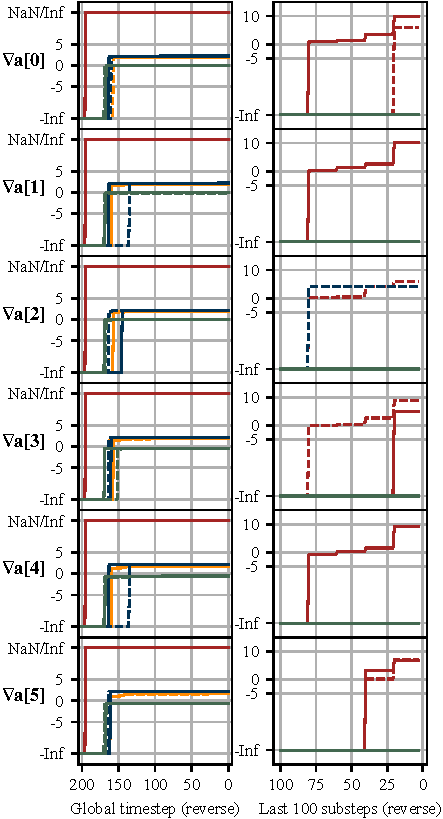
\includegraphics[width=\columnwidth]{images/grads/action-res40.pdf}
\caption{Actions (6D)}\label{subfig:grad-action}
\end{subfigure}\\
\begin{subfigure}{0.48\columnwidth}
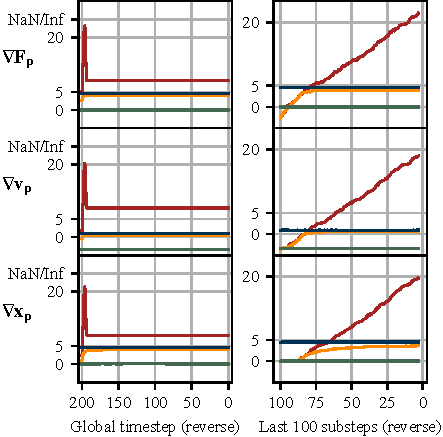
\includegraphics[width=\columnwidth]{images/grads/p-res40.pdf}
\caption{Particle variables (deformation gradient, velocity and position)}\label{subfig:grad-p}
\end{subfigure}\hfil
\begin{subfigure}{0.48\columnwidth}

\includegraphics[width=\columnwidth]{images/grads/grid-res40.pdf}
\caption{Grid variables (mass, velocity before and after collision detection)}\label{subfig:grad-grid}
\end{subfigure}
\caption{\label{fig:ggrads}The log scale (base $10$) of the gradients of the key MLS-MPM variables, physics parameters, and actions from the last global timestep to the initial timestep (left side of each subfigure) as well as in the substep scale for $100$ substeps (right side of each subfigure). A global timestep $= 20$ substeps. Solid lines represent the maximal value and dash lines the minimal value of the gradient vector.}
\end{figure}

\rp{It is clear from the red lines (with no gradient operations) that the scales of the gradients grow sharply while back-propagating within $100$ substeps ($5$ global steps) and eventually result in $NaN$s or numerical infinities. On the other hand, with the three gradient operations, these gradients can be kept within a reasonable scale ($[-5, 5]$), as shown by the orange, blue, and green lines, corresponding to the clipping, dynamic scaling, and normalisation operations, respectively. This indicates the effectiveness of the three techniques in constraining the gradient scales of the key MLS-MPM variables, thus ensuring stable gradients for optimising the physics parameters and actions.}

Figure~\ref{fig:loss-grad-app} shows the loss landscapes and the approximate gradients of the system identification task over Poisson's ratio and sand friction angle dimensions (top) as well as the second, third and fourth skill parameters for the first digging task (bottom). These results are also obtained with sampling resolutions $20$, $40$ and $60$. Similar to the analyses in subsection III-F, it can be seen that HMD tends to produce smoother loss landscapes, indicated by the observation that the HMD gradients are less noisy.

\begin{figure*}
    \centering
    \begin{subfigure}{\linewidth}
    \centering
    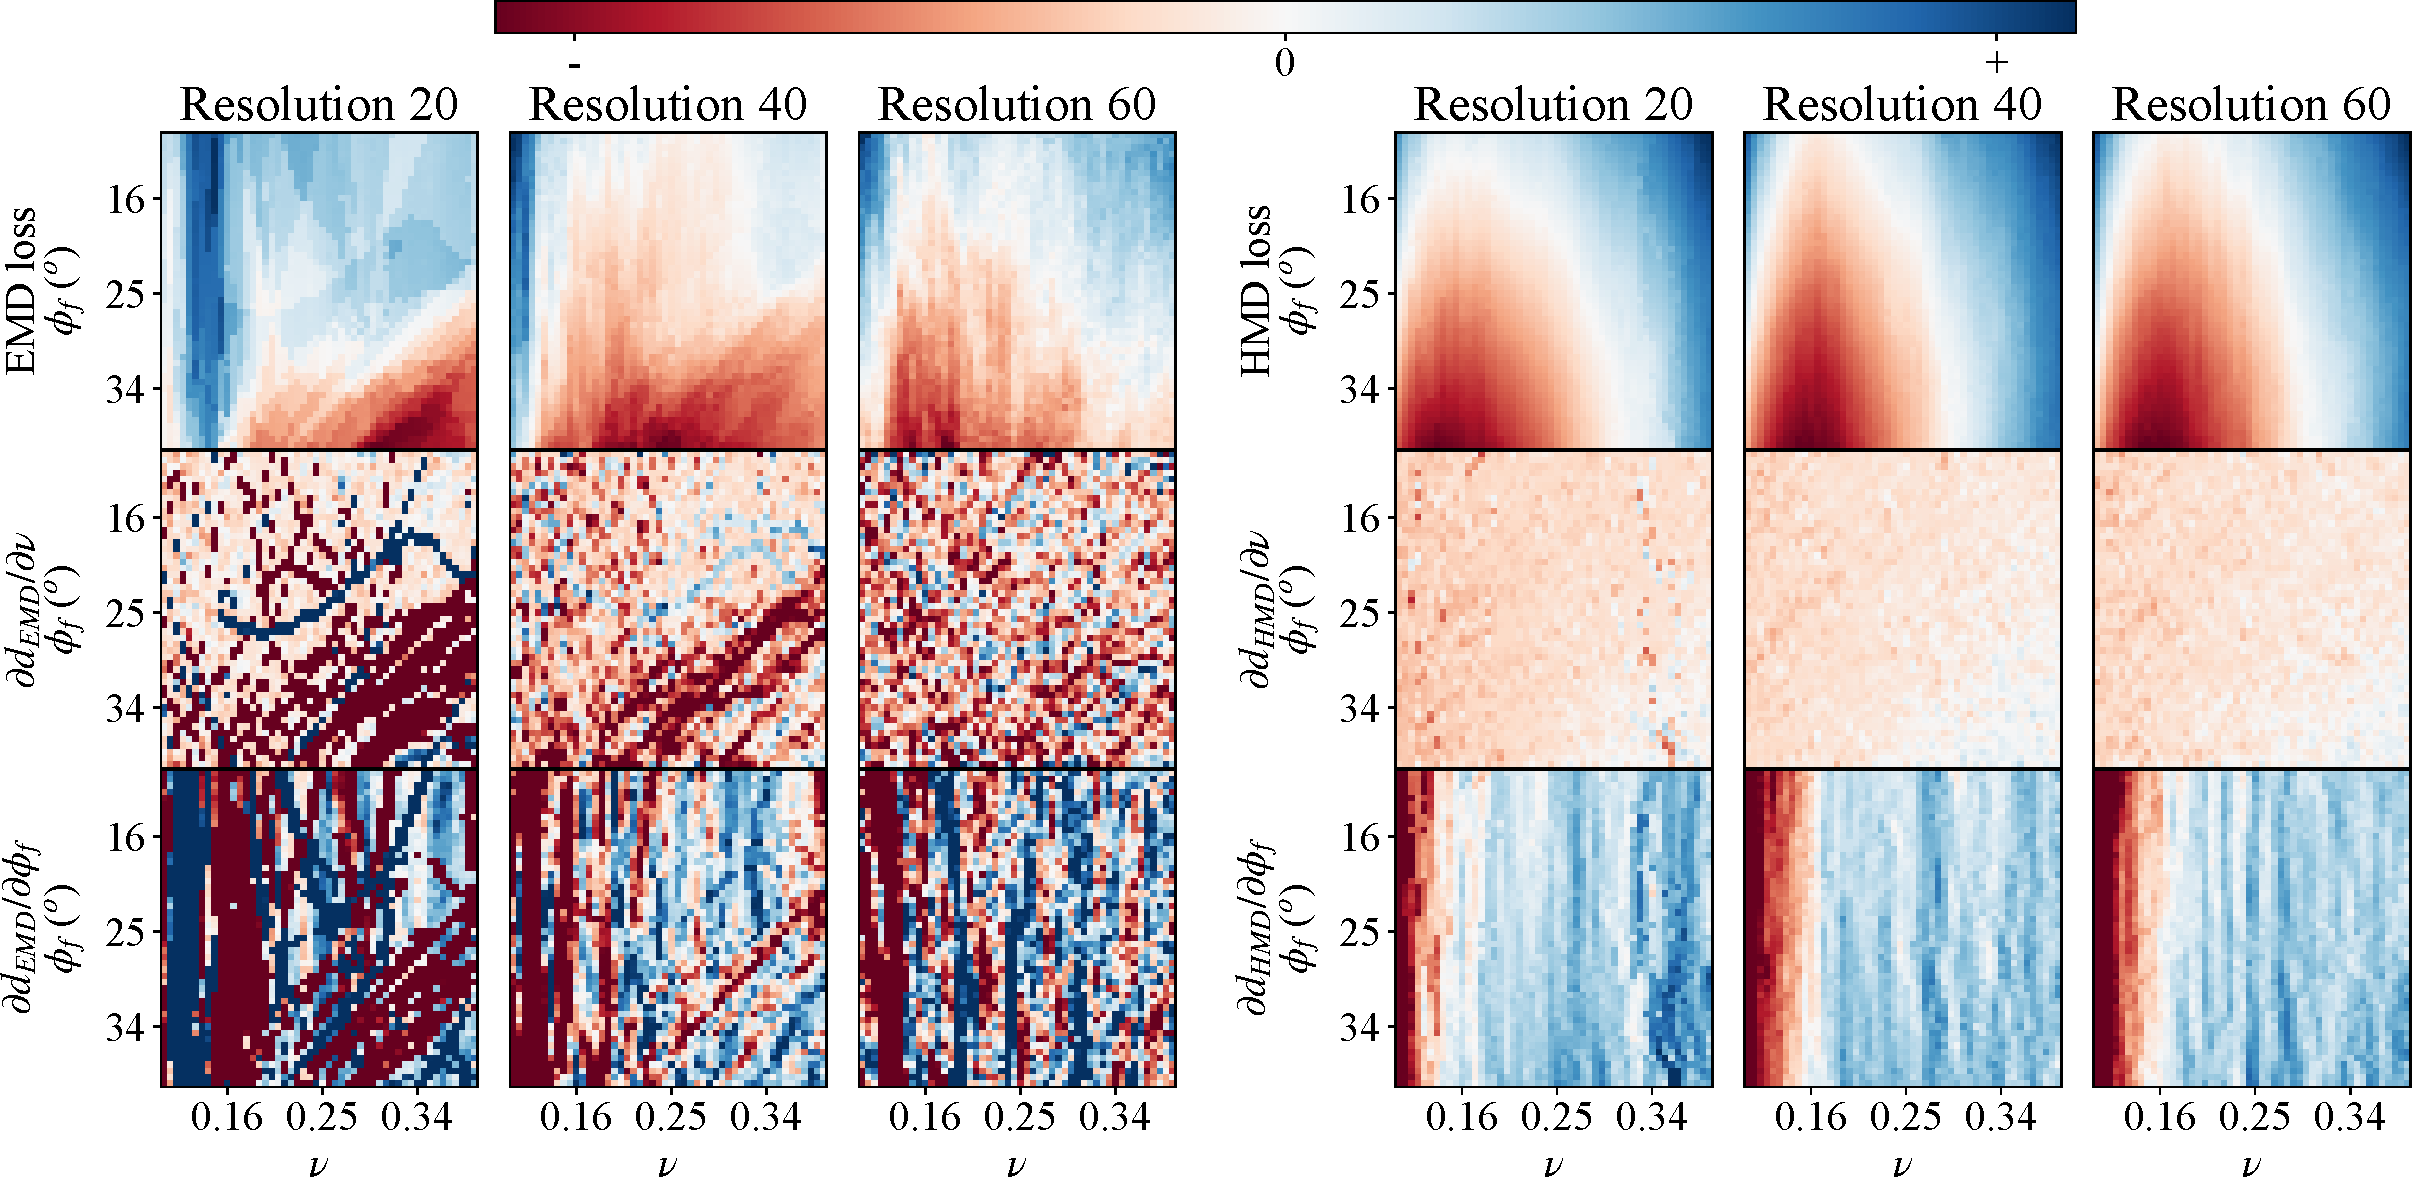
\includegraphics[width=0.9\linewidth]{images/losses/NS-losses-grad.pdf}
    \caption{System identification task. On Poisson's ratio and sand friction angle.}\label{subfig:NS-loss}
    \end{subfigure}\\
    \begin{subfigure}{\linewidth}
    \centering
    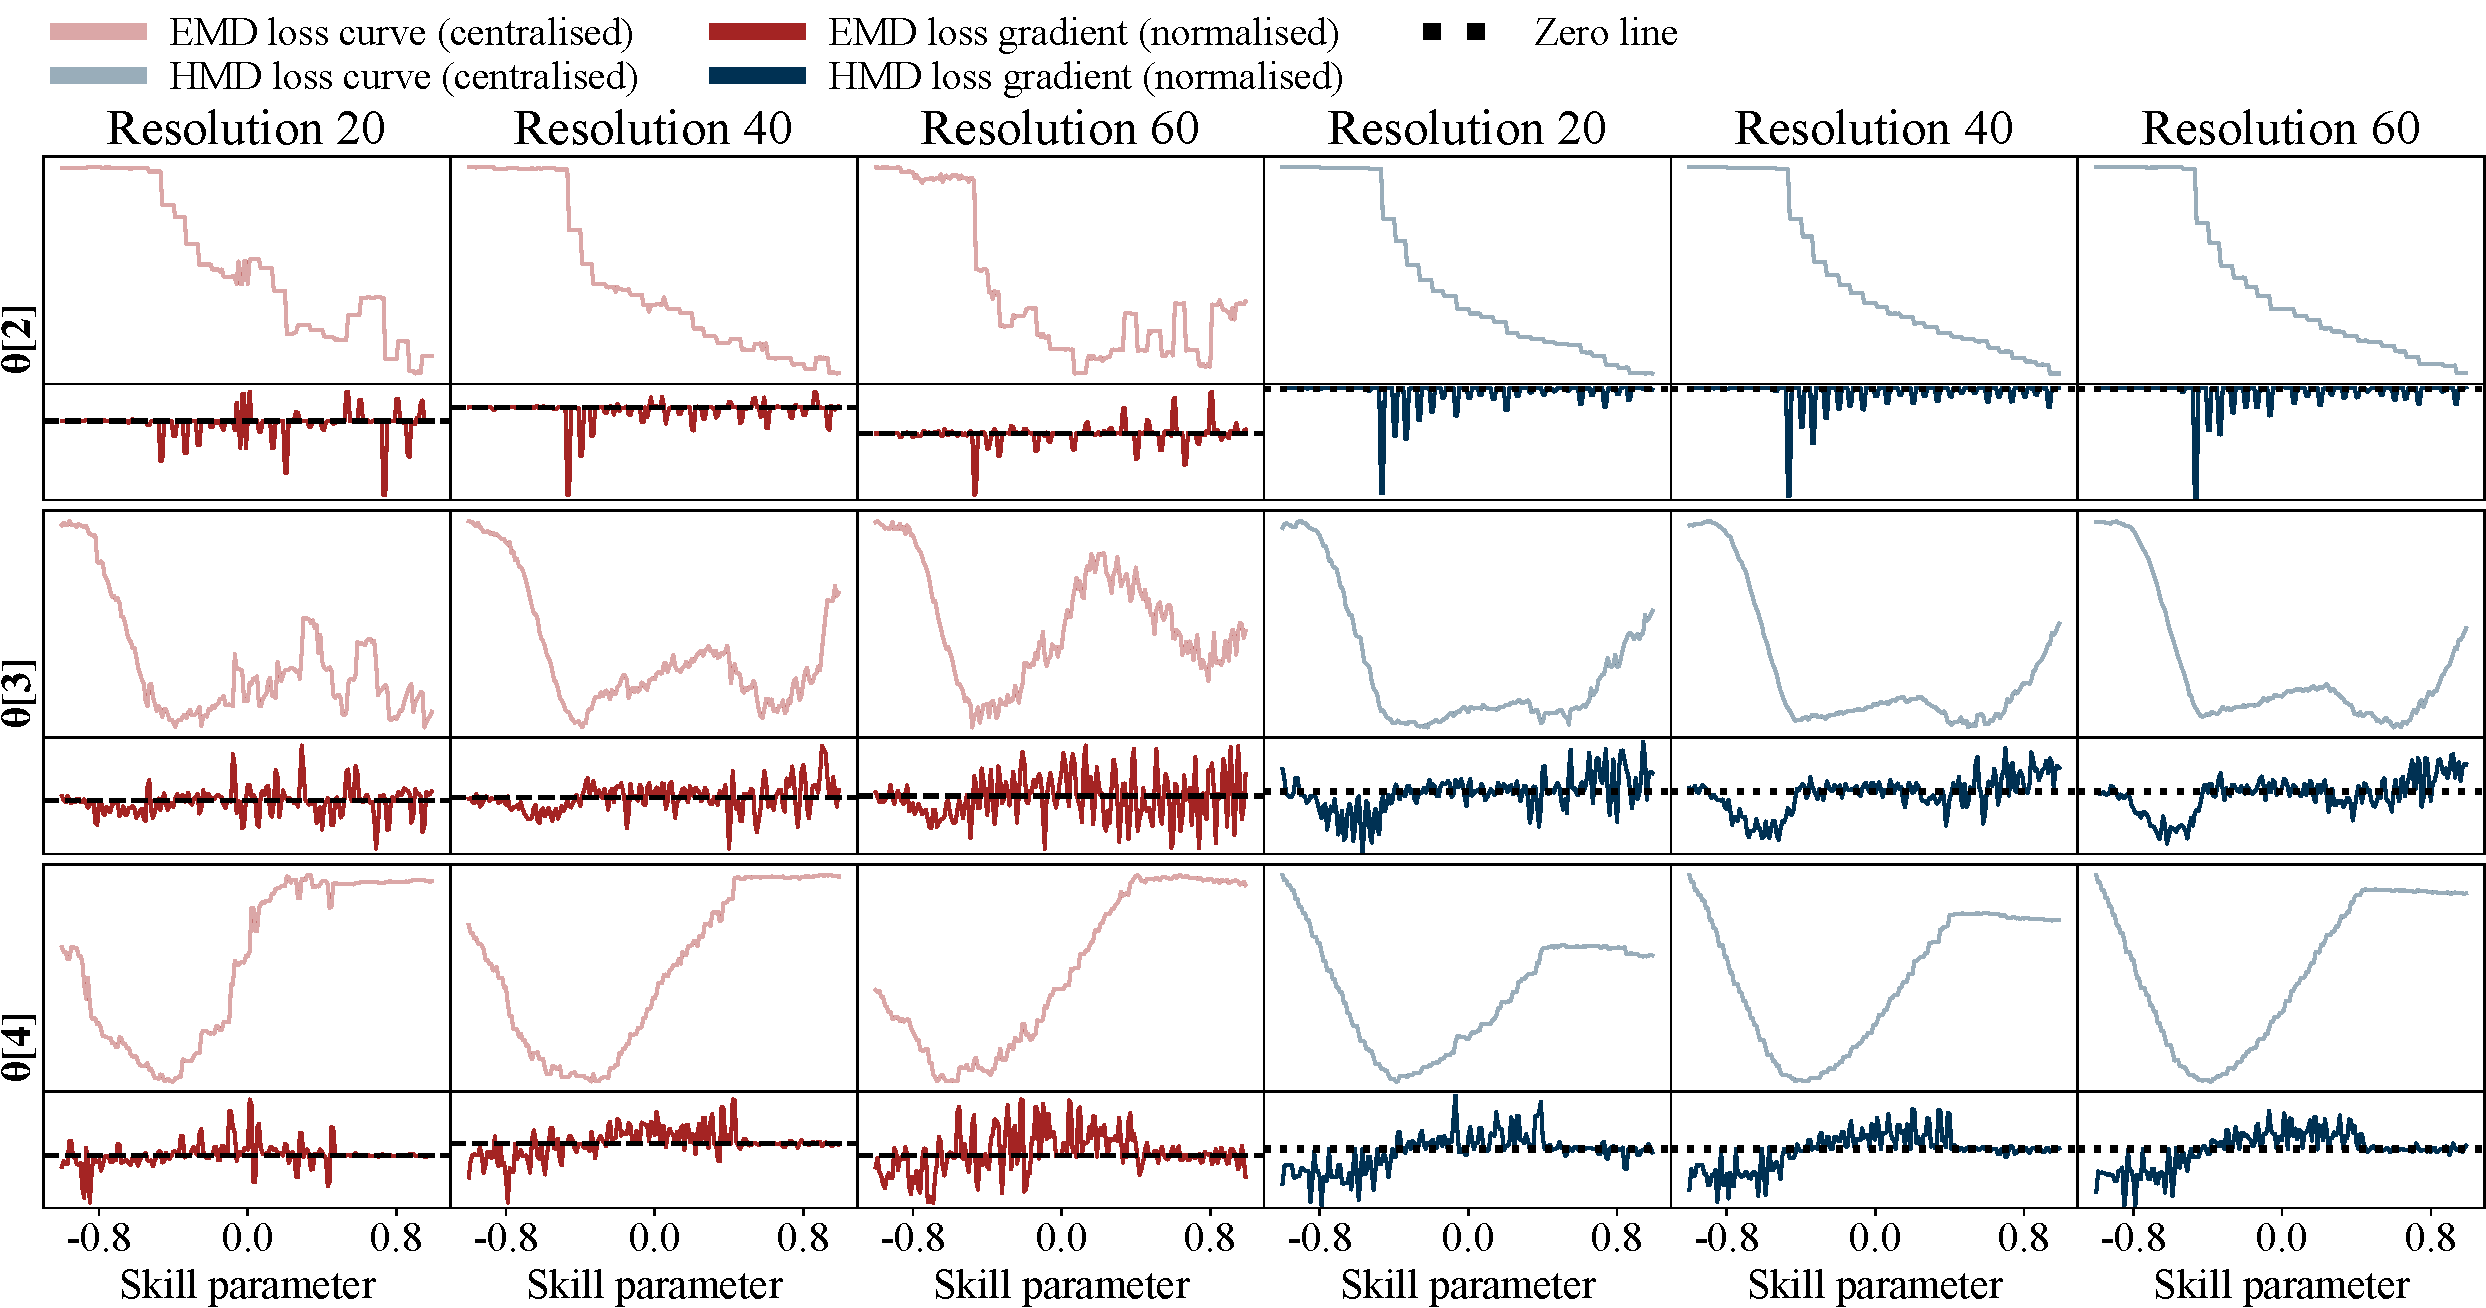
\includegraphics[width=0.89\linewidth]{images/losses/skill-losses_.pdf}
    \caption{Skill optimisation task. On skill parameter $2$, $3$ and $4$.}\label{subfig:skill-loss-1}
    \end{subfigure}
    \caption{Loss landscapes and their gradient distributions.}
    \label{fig:loss-grad-app}
\end{figure*}

\section{Training statistics of the reinforcement learning agent}
Figures~\ref{fig:stat-rl-0}, \ref{fig:stat-rl-1}, and \ref{fig:stat-rl-2} present the detailed statistics of the goal-conditioned SAC agent on the three soil digging tasks. In three tasks, the increased actor losses (estimated Q values), the decreased critic losses and the stabilised policy entropies indicate that the algorithms have converged. The EMD and height map losses, however, indicate that the algorithm could only find good solutions in task 1 while it failed at the other two tasks (this was also observed in Figure 10a).


\begin{figure*}
    \centering
    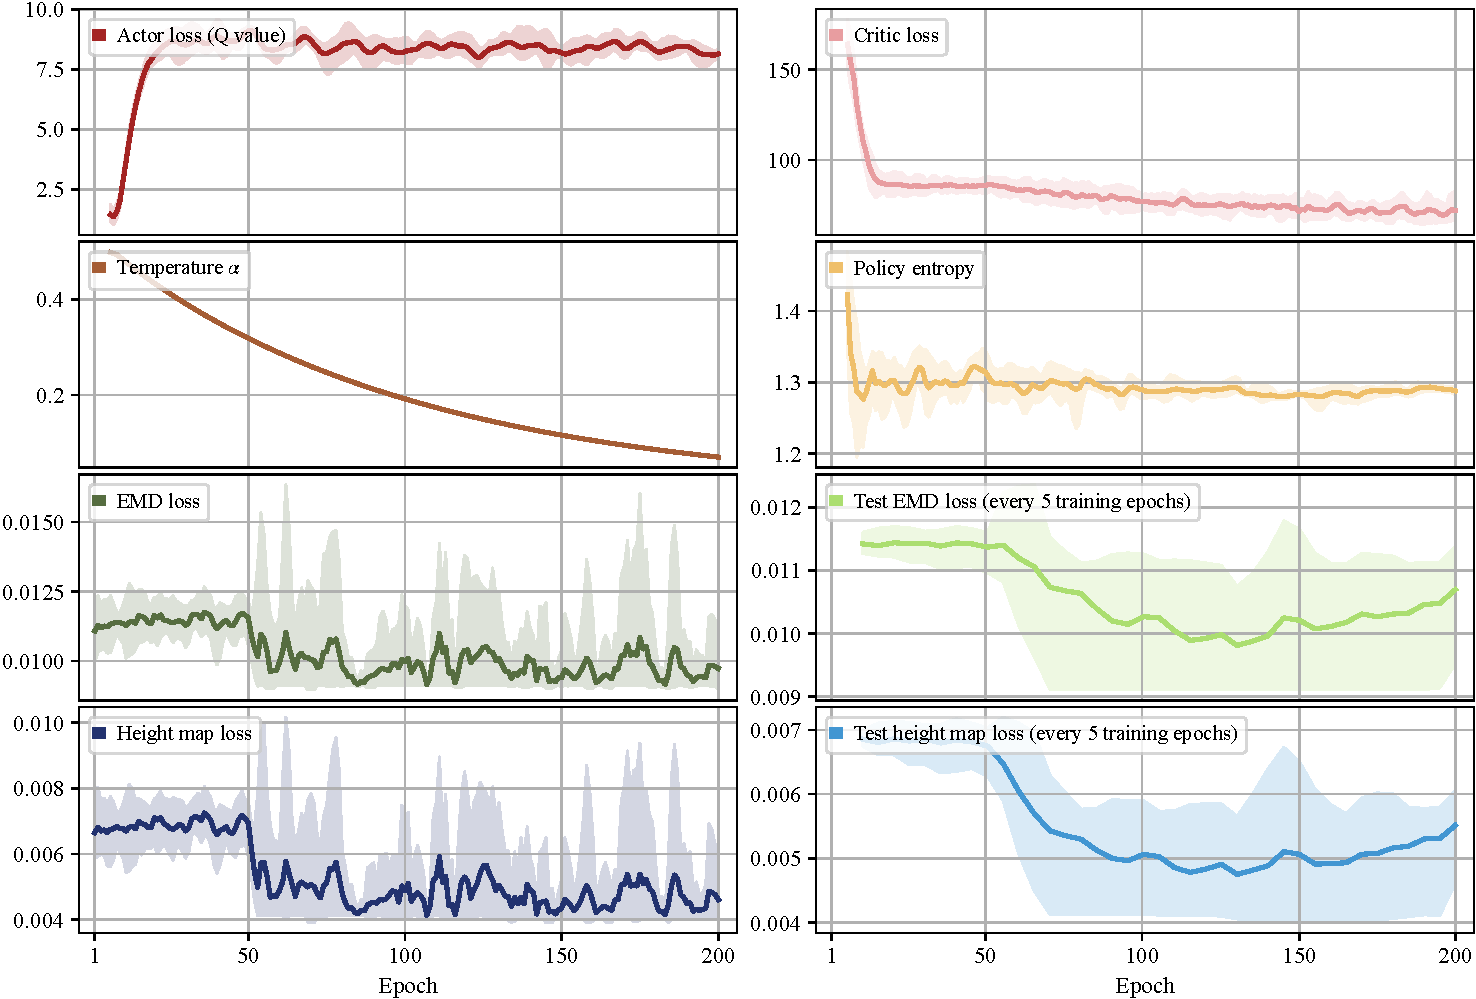
\includegraphics[width=0.9\linewidth]{images/rl_task0.pdf}
    \caption{Goal-conditioned SAC training statistics on soil task 1.}
    \label{fig:stat-rl-0}
\end{figure*}

\begin{figure*}
    \centering
    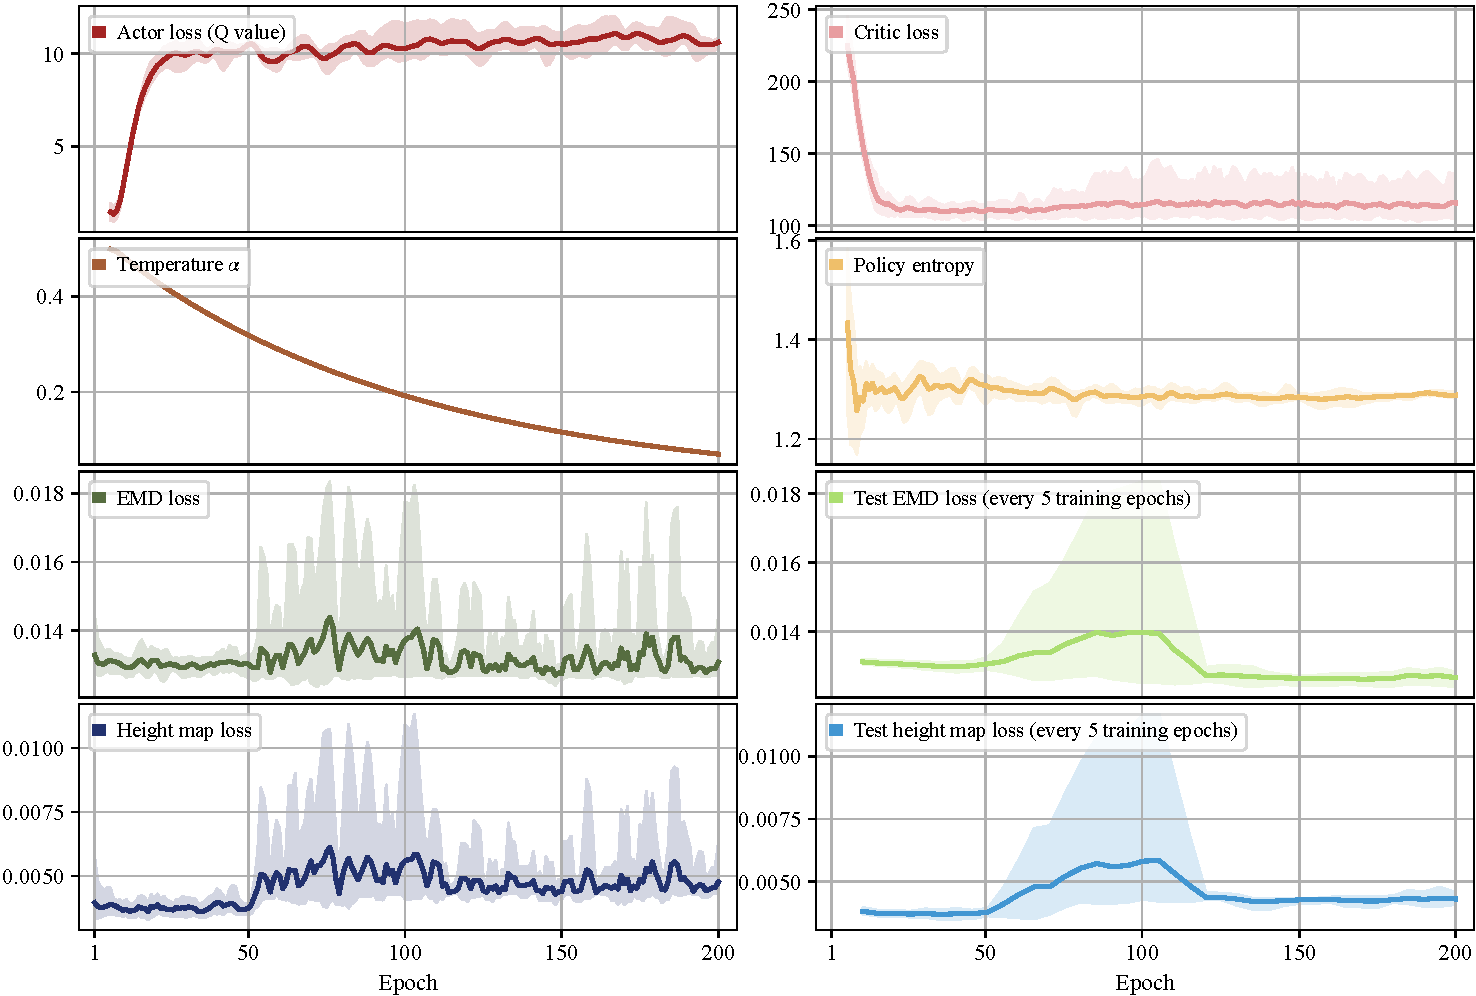
\includegraphics[width=0.9\linewidth]{images/rl_task1.pdf}
    \caption{Goal-conditioned SAC training statistics on soil task 2.}
    \label{fig:stat-rl-1}
\end{figure*}

\begin{figure*}
    \centering
    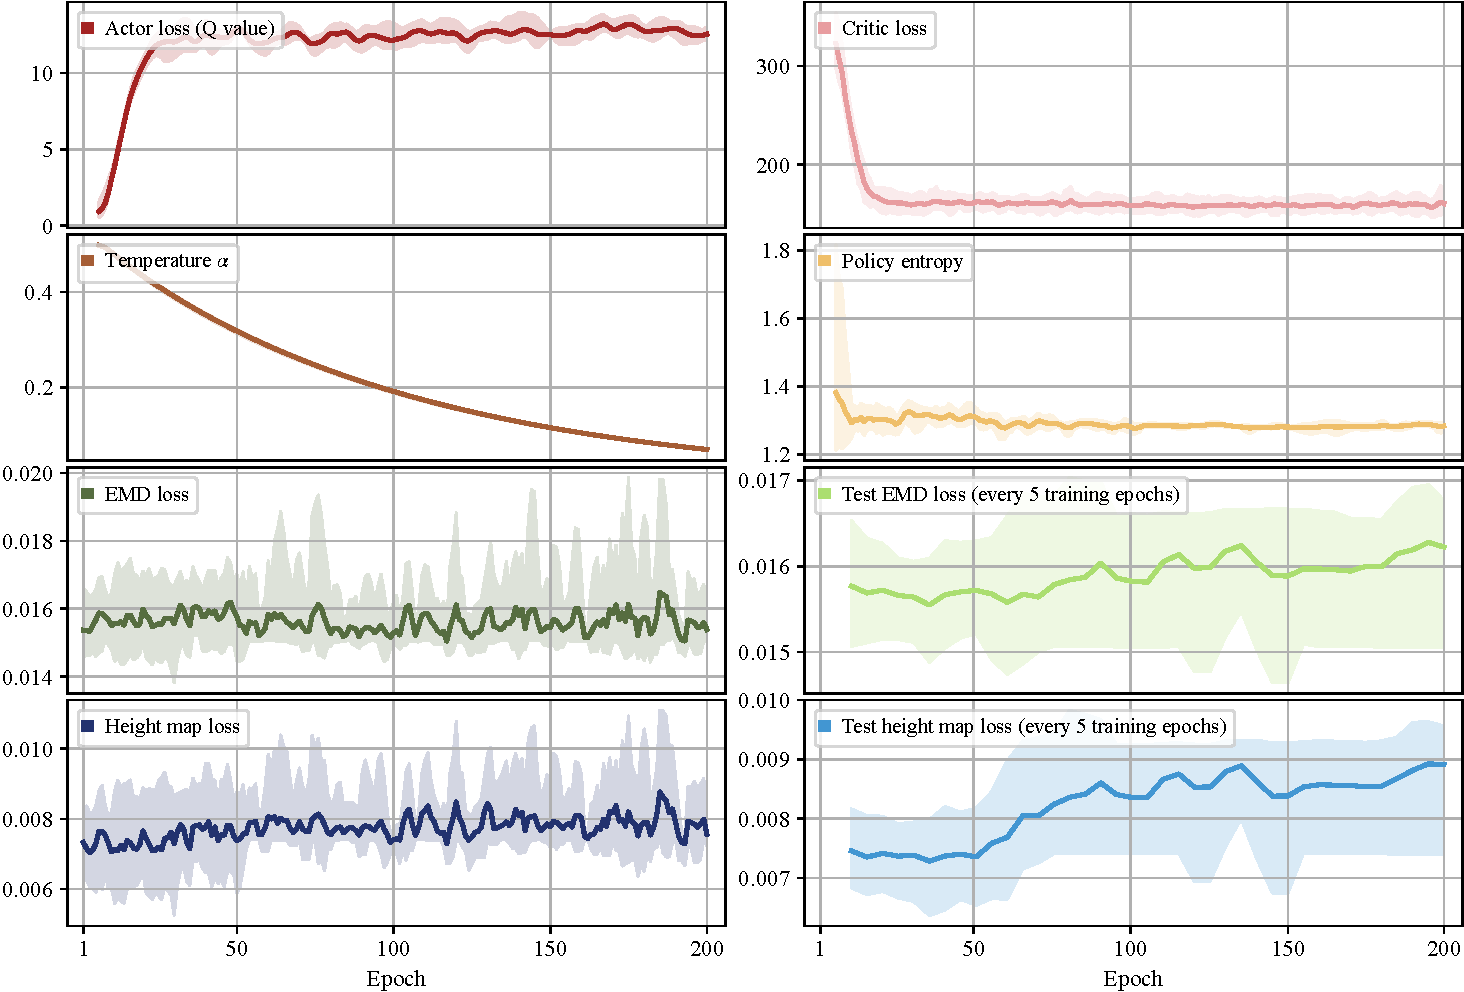
\includegraphics[width=0.9\linewidth]{images/rl_task2.pdf}
    \caption{Goal-conditioned SAC training statistics on soil task 3.}
    \label{fig:stat-rl-2}
\end{figure*}

\printbibliography

\end{document}
